\documentclass[11pt]{book}
\usepackage{geometry}      
\geometry{letterpaper}    
\usepackage[parfill]{parskip}  
\usepackage{graphicx}
\graphicspath{ {images/} }
\usepackage{amssymb}
\usepackage{amsmath}
\usepackage{epstopdf}
\usepackage{float}
\usepackage{adjustbox}
\usepackage{listings}
\usepackage{tabto}
\usepackage{gensymb}
\usepackage{nameref}
\DeclareGraphicsRule{.tif}{png}{.png}{`convert #1 `dirname #1`/`basename #1 .tif`.png}

\usepackage[colorlinks=true, pdfstartview=FitV, linkcolor=blue, 
            citecolor=blue, urlcolor=blue]{hyperref}



\newtheorem{theorem}{Theorem}
\newtheorem{corollary}[theorem]{Corollary}
\newtheorem{definition}{Definition}
\newtheorem{lemma}{Lemma}
\newtheorem{exercise}{Exercise}
\newtheorem{remark}{Remark}
\newtheorem{example}{Example}
\newtheorem{warning}{Warning}
\newcommand{\gdgas}{GDELT\_GA\_Search\ }

\def\grad{ \mbox{grad}}
\def\curl{ \mbox{curl}}
\def\div{ \mbox{div}}
\def\U{\ensuremath {\cal U}}
\def\S{\ensuremath {\cal S}}
\def\V{\ensuremath {\cal V}}
\def\R{\ensuremath {\cal R}}
\def\tr{\ensuremath {\mbox{tr}}}




% ------------------- Title and Author -----------------------------
\title{GDELT GA Search Users Manual}
\author{User's Guide and Manual}
\begin{document}


\frontmatter
\maketitle

\tableofcontents

\mainmatter
%!TEX root =  GDELT_GA_Search_UsersManual.tex

\chapter{Introduction} \label{chap:Introduction}
\par GDELT is the Global Database of Events, Language, and Tone, a record of real-world events  harvested automatically from world news sources. Its records begin from 1979 and continue to the present, and the most recent versions of the GDELT data set are updated every 15 minutes. The records are compiled using natural language processing (NLP), and the record for each event includes not only information about the actors and actions, but also about aspects of how the action is described and discussed in the news: how widely, for how long, in what tone, etc. Consequently, GDELT provides an incomparable record of how events in the real world are being considered and expressed by the general public.

\par At a micro-level, a record in the GDELT data set is able to shed light on how a specific event was considered. For example, the GDELT data set shows whether an event was discussed widely or only briefly, whether it was discussed while it ocurred or only afterwards, whether it was debated or celebrated, or whether it was memorialized and recalled long after it first took place. At a macro-level, the complete record of GDELT events forms a richer data source, one that can inform about long-term dynamics and ongoing world historical processes, of which individual events are only single lines in a longer play.

\par A difficulty, however, is that the complete GDELT data set covers the whole world: it is more than just one play; it is a whole library. The challenge is often to find the correct level at which to understand the story that GDELT is telling. More formally, one might wish to isolate specific subsets of the GDELT data that apply to an area of interest and to leave out all of those that do not.

\par GDELT is integrated with a query search that can extract subsets based on the data contained in GDELT's records. For example, if one were interested in diplomacy between France and Russia in 2018, one could perform a search in which those two countries are listed as `actors' and the time range was limited to the period of interest of 2018. Other filters (for example, actions of specific kinds) could also be applied. However, for some purposes, it may be difficult to guess at what is the proper query because false positives and false negatives can dominate, washing out the signal.

\section{Finding Relevance: A GA Approach}

\par The \gdgas toolkit assumes that there can be valuable relationships between subsets of GDELT data and other time-series data found in the real world. The canonical example is that bursts of activity in global news reporting concerning some ongoing process (e.g., a world conflict) will be echoed by similar activity on social media platforms. Because of this relationship between news and social media, time-series showing activity on these social media platforms should be able to be related to a time-series showing discussions in world news events as catalogued by GDELT. 

\par An additional expectation is that these relationships will only be visible on specific subsets of the GDELT data. The global number of news articles collected by GDELT and the number of events catalogued will remain more or less constant, but the content will vary through time. The subset of content that is of interest will be unified by some common element such as a specific term, a set of terms, or even other criteria. The challenge is to find the criteria that, when issued as a query against the full GDELT data set, returns a set that has a signature related to the long-term issue being considered.

\par For example, the four graphs in figure \ref{FourGraphsFigure} show time series data with time on the x-axis. The upper graph represents the activity on some social media platform: activity is low early in the period shown, then there is a burst followed by heightened activity, and there is a drawdown through the remainder of the period.

\par The second graph from the top shows the total GDELT events. Note that this graph would already have been subselected using keywords. (Although the \gdgas toolkit can work with the entire GDELT data set, upstream preprocessing like this is common to winnow the GDELT data to only elements likely to be relevant.) The key aspect here is the alignment with the upper graph. Notice that there is a sharp burst and then a drawdown that shows a strong correlation between the graphs. Even so, the alignment is far from exact. (Note also that scales would be omitted from the axes. It is assumed that the x-axes are the same, but this is not true for the y-axis: the number of events in the upper graph may be in the millions while the number in the lower graph is in the thousands. What matters is their correlation.)

% re-do graph, needs to be a, b, c, and d of Fig. 1
% top graph maybe supposed to be SOCMED or SocMED? JTM: YES, it was supposed to be 'Social Media' or 'SocMed' or something...
% In this graph the match between top and bottom is perfect, because these are fake data, but if we re-do the graphs to use real data (hence imperfect) we can reword some of the description below. 
\begin{figure}
[htbp] 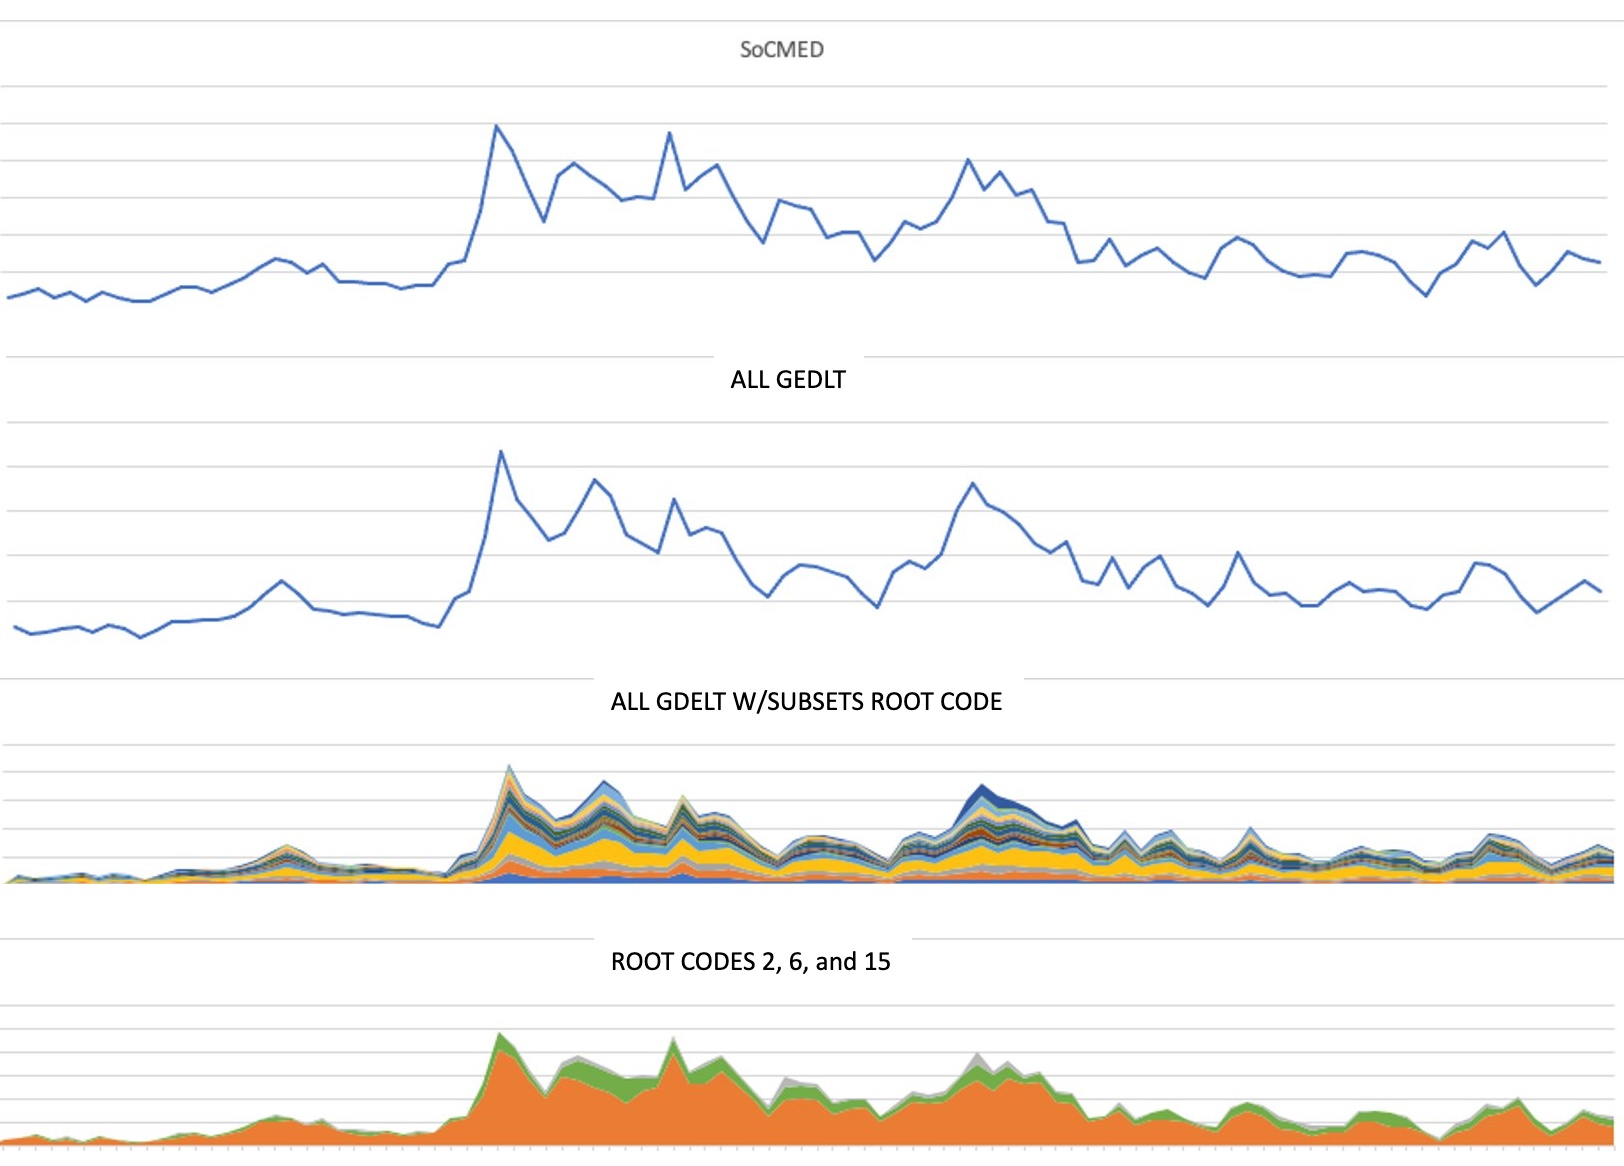
\includegraphics[width=\columnwidth]{TheoryGraphs.jpg}
\caption{Conceptual view of the search process} 
\label{FourGraphsFigure} 
\end{figure}

\par The ALL GDELT W/SUBSETS ROOT CODE graph (c) shows the same graph as (b); however, where (b) showed only the total, (c) subdivides the GDELT data---in this case, by the value for \textit{root code} (see below). There are 20 possible values for this field, and hence 20 bands in the graph. Each band represents the counts of GDELT events with the specified root code. 

\par The lowest graph (d) shows the results when only three root codes (2, 6, and 15) are included in the GDELT totals. Whereas the graph of all the GDELT events matches the social media event graph at a general level, the graph of these three specific root codes matches much more closely. 

\par This offers a nice example the \gdgas toolkit because it is easily bounded: with 20 root codes, there are exactly ${2^n - 1}$ combinations possible. For 20 root codes this is 1,048,575 combinations. This would be manageable with a brute-force approach---it is not difficult to try 1 million combinations---but this number grows quickly as more possible criteria are added. It is easy to reach a space that is too large to explore fully, so a different approach is needed instead.

\par The \gdgas tool searches through this space by building GDELT time series using \textit{queries}. A query is a set of criteria that serve to classify the GDELT data and extract matching events. The crux of the \gdgas algorithm is that these queries can be changed in an iterative way that moves through the search space. The algorithm is this:

\begin{itemize} 
	\item \textbf{Construct a query framework} that extracts subsets of GDELT data based on an array of possible fields 
	\item \textbf{Score the results} based on the information they provide about the social media time series
	\item \textbf{Mutate the best-scoring variations} to explore whether expanding or reducing the criteria improve the scores
\end{itemize}


\section{Acknowledgements}
%specific text that we have to use to acknowledge funders
%The funders (DARPA), the creators, the team, etc.


% Note: GDELT documentation indicates that some events are reciprocal: "Biden meets with Putin" would have a matching event, "Putin meets with Biden." These should show up as identical events but with the actors reversed; see https://www.gdeltproject.org/data/documentation/CAMEO.Manual.1.1b3.pdf, p. 8, CAMEO '019', "Express Accord". I have never found an example of this; GDELT does not link these together (they would be separate records), and it is unclear if every entry in the 'mentions' table would be duplicated as well.



% Let's save all of this for later in the document
% \par Test history is taken from 'test unknown'. See how good it does scoring things more than once to be sure it does not do well once by chance. %scoring what?
% \\The genetic algorithm operates through iterations. Iterations are given graph improvement scores over run-time. This is because there is a cost-benefit analysis for continuing to run. %make more clear
%Not sure what was planned below, plus hypperrefs don't work. 
%\par  \hyperref[sec:4]{To construct a query framework}
% \\Queries are methods of passing through data and finding subsets. Queries can contain other queries and the results can be added together and weighted.
%\par \hyperref[sec:3]{To construct a query framework} to score the results %add
%\par To mutate the best-scoring variations%add



% Let's also save this for later in the document
% Some fields \textit{completely determine others in the entire GDELT data set}. 
% For example, \emph{MonthYear} is merely a reformatted version of \emph{day}; whereas \emph{day} is in YYYY-MM-DD format, \emph{MonthYear} is in YYYYMM format. 
% So, if \emph{day} is known, then \emph{MonthYear} can be derived. 
%In many cases, searching on both fields would be redundant (although it may also be the case that a combination of search strategies might be better than searching just one field using one strategy).

% It may also be the case that some fields completely determine others \textit {within a specific subset of GDELT data}. For example, if a data set is drawn from a date range that begins %December 1st of 2010 and ends January 31st of 2011, then any record with a \emph{Year} value of 2010 must have a \emph{MonthYear} value of ``201012", and any record with a \emph{Year} value of 2011 must have a \emph{MonthYear} value of ``201101''. This, however, is an attribute of the subset of data use rather than the way that the GDELT data set has been constructed. It may be useful in specific applications, but not in the general case, it is not addressed further here.

 %!TEX root =  GDELT_GA_Search_UsersManual.tex

\chapter{Getting Started: Running \gdgas Searches} \label{chap:Running}

This chapter provides a basic introduction to running the simulation 	

\section{Input Data}
The input data for \gdgas searches consists of four kinds of files:

\begin{itemize}
\item GDELT Data, including:
\begin{itemize}
\item Events Data
\item Mentions Data (can be omitted)
\end{itemize}
\item Time Series Comparative Data
\item The GDELT Properties File
\item Run Group Specification File (for sets of parallelized runs)
\end{itemize}

The GDELT Properties File and the Run Group Specification File are used with single runs and with parallelized runs, which are both discussed in subsequent sections

\subsection{GDELT Data}
GDELT data consists of \textit{events} and \textit{mentions}. Both of these are given in CSV files downloadable from GDELT's archives. This toolkit provides a pair of tools that can automatically download events and related mentions from within a given time frame. (Note that mentions may accumulate after the initial event, and thus some events' mentions may fall outside the original time limit for events). An alternative data structure in JSON, from the original project for which this tool was designed, is also accommodated but is not documented.

\subsection{Time Series Comparative Data}
The search will compare the GDELT data with a time series; the input data for the time series has the following structure (for more information, see \ref{TimeSeriesDataStructure}).

\begin{verbatim}
platform,frame,ConvertedDate,counts
twitter,capitol,2020-10-01,1034
twitter,capitol,2020-10-02,1081
twitter,capitol,2020-10-03,1096
twitter,capitol,2020-10-04,1116
twitter,capitol,2020-10-05,1198
twitter,capitol,2020-10-06,1234
twitter,capitol,2020-10-07,1271
twitter,capitol,2020-10-08,1368
etc.
\end{verbatim}


\section{Running Single Runs}

\subsection{The GDELT properties file}\label{sec:GDELTPropertiesFile}

The GDELT properties file describes the location of the GDELT data, its chronological boundaries, the parameters of the GDELT queries (including their mutation properties), the location of the social media data, and some other properties of exploration. The structure of the file is simple: each line can contain one property specification, with a non-whitespaced property name on the left, an equals sign, and the property value on the right. Lines that start with number signs are ignored and can be used as comments.

Here is an example of a file

\begin{lstlisting}
# GIT DIRECTORY
gitDir = /home/username/gdelt_ga_search

# GDELT DATA FILE LOCATION AND INFO
dataLocation     = ./data/examples/GDELT_Events_Data.csv
mentionsLocation = ./data/examples/GDELT_Mentions_Data.csv
beginHistory     = 2020-01-31
dayZero          = 2021-01-01  

# GDELT QUERY SPECIFICATIONS
MaxShift              = 24
MinShift              = 24
MaxVizOffset          = 0
MinVizOffset          = 0
Actor1CountryCodes    = null,KEN,ZWE,UGA,AFR
Actor2CountryCodes    = null,KEN,ZWE,UGA,AFR
MatchGoldsteinScale   = FALSE
MatchAverageTone      = FALSE
MatchRootCode         = FALSE
MatchLatLon           = FALSE

# MUTATION WEIGHTS
Actor1CountryCodesMutateWeight = 10
Actor2CountryCodesMutateWeight = 10

# TIME SHIFT MUTATION PROBABILITY
MutatingTimeshiftProb           =  0

# TIME SERIES DATA FILE LOCATION AND INFO
timeSeriesDataLocation = ./examples/DummySocialMediaCounts.csv
timeSeriesDataStart    = 2020-10-01T00:00:00

# BAILOUT
bailoutInterval  = 3600
bailoutValue     = 100
\end{lstlisting}

\begin{itemize}
\item \textit{gitDir} This specifies the directory of the GDELT code. In cases where the code may be modified, it can be useful to employ a mechanism that will stop a run if the code has not been committed.
\item \textit{dataLocation} The location of the GDELT events data file.
\item \textit{mentionsLocation} The location of the GDELT mentions data file. This can be omitted if no mentions are available
\item \textit{beginHistory} The earliest date in the GDELT data
\item \textit{dayZero} The date that will be considered the boundary between training and prediction  
\item \textit{MaxShift} Maximum number of hours the GDELT search will `shift' times. This can be used so that predictions are not (or, occasionally, are) based on information from the future, e.g. a 24-hour shift means the predictions are based on the day prior.
\item \textit{MinShift} Minimum number of hours to shift. If this value is the same as the MaxShift, the shift will be constant
\item \textit{MaxVizOffset} Maximum visibility offset, or the number of hours offset the visibility of events will be
\item \textit{MinVizOffset} Minimum visibility offset
\item \textit{Actor1CountryCodes} List of country codes that are used for Actor 1 Country Code queries
\item \textit{Actor2CountryCodes} List of country codes that are used for Actor 2 Country Code queries
\item \textit{MatchGoldsteinScale} Whether to consider Goldstein Scale when matching queries
\item \textit{MatchAverageTone} Whether to consider Average Tone when matching queries
\item \textit{MatchRootCode} Whether to consider Root Code when matching queries
\item \textit{MatchLatLon} Whether to consider Latitude and Longitude when matching queries
\item \textit{Actor1CountryCodesMutateWeight} Weighted probability that the Actor 1 Country Code element of a query will mutate
\item \textit{Actor2CountryCodesMutateWeight} Weighted probability that the Actor 2 Country Code element of a query will mutate
\item \textit{MutatingTimeshiftProb} Probability that the shift value will mutate
\item \textit{timeSeriesDataLocation} File location for the social media counts
\item \textit{timeSeriesDataStart} Earliest date in the social media files.
\item \textit{bailoutInterval} Time (in seconds) after which the routine will stop a search if no improvement has been found
\item \textit{bailoutValue} Number of iterations after which the routine will stop a search is no improvement has been found
\end{itemize}

\subsection{Using the Runner Class from the Command Line}

It is possible to use the Runner class to run single runs of the search. This requires a collection of arguments. A typical command line will include arguments following this example:

\begin{itemize}
\item \textit{ /usr/lib/jvm/java-8-openjdk-amd64/bin/java}  is the path to the Java RunTime
\item \textit{ -DGDELT\_GAS\_PSCRIPT\_PATH=``/home/gdelt\_ga\_search/pscripts/"}  is the path to the Python Scripts. This is required even if Python Scripts are not used
\item \textit{-Dfile.encoding=UTF-8} A specification of file encoding
\item \textit{-classpath ./bin:./lib/gson-2.8.5.jar:./lib/jeromq-0.4.0.jar:./lib/commons-math3-3.6.1.jar gdelt.runners.Runner} The classpath
\item \textit{RUNNER\_0} An identifier that is used for some interim files
\item \textit{./examples/SampleConfig.props} The properties file in which the characteristics of the input data and queries are specified
\item \textit{LINEAR\_REGRESSION} The type of prediction to be used
\item \textit{NRMSE\_MEAN} The type of scoring to be used
\item \textit{2021-01-01} The date to be used as day zero
\item \textit{28} The duration of the training period
\item \textit{21} The number of days forward to predict for the final prediction
\item \textit{21} The number of days to predict for the training periods
\item \textit{50 }The population size
\item \textit{10} The number of survivors
\item \textit{15} The number of generations to run if no stopping condition is encountered
\item \textit{7} The number of days prior to day zero minus the test prediction period to take as the training period day zero
\item \textit{twitter\_capitol} the data source ('platform') and topic ('frame') to be used; must match the input data given in the configuration properties file named above 
\item \textit{DEMO\_001\_000000::NewQueries} An alphanumeric identifier and a description; the description can use underscores as spaces. The description will be written with every output file.
\end{itemize}

\section{Running Parallelized Suites of Runs}

\subsection{The Run Group Specification File}

The Run Group Specification File contains the information needed to structure a collection of parallelized runs. The format is a property on the left, a pair of colons, and a value on the right. The term on the right may include several different values. The configuration will create a set of runs based on all of the possible combinations of values.

An example listing of a Run Group Specification File (from ./examples/SampleConfig.props).
\begin{lstlisting}
predMethods::LINEAR_REGRESSION
scoreMethods::NRMSE_MEAN
zeroTimes::2021-01-01
trainDurations::28
predDurations::21
predDurationTrains::21
popSizes::50
survivorValues::10
generations::15
predictionPoints::7,0
platforms::twitter,youtube
frames::capitol,insurrection
\end{lstlisting}

The meanings of these are:

\begin{itemize}
\item \textit{predMethods} The method to be used for prediction; valid values are the names of the values in the PREDICTION\_METHOD enum of the Predictor class.
\item \textit{scoreMethods} The method of scoring to be used; value values are the names of the values in the SCORE\_METHOD enum of the Scorer class.
\item \textit{zeroTimes} Times that are to be used as the boundary between training and prediction
\item \textit{trainDurations} Number of days that are used for training periods
\item \textit{predDurations} Number of days forward (ahead of zero time) that is considered prediction
\item \textit{predDurationTrains} Number of days forward used by the training samples. 
\item \textit{popSizes} Size of the GA population
\item \textit{survivorValues} Number of best-scoring survivors in the population
\item \textit{generations} Number of generations the search will run if it does not hit a stopping condition first
\item \textit{predictionPoints} Days prior to zero time \textit{minus the predDurationTrains} value that will mark the train/test boundary for the predictions.
\item \textit{platforms} Social media platforms to be explored
\item \textit{frames} Frames (topics) to be explored
\end{itemize}

In the above example, eight combinations would be created based on the fact that multiple values for prediction points, platforms, and frames are combined.

\subsection{Running The ParallelMultiRunner Class from the Command Line}

When running the ParallelMultiRunner from the command line, the arguments should be
\begin{itemize}
\item The full path to your Java runtime, e.g. /usr/lib/jvm/java-8-openjdk-amd64/bin/java 
\item The relative path to your GDELT Properties file, e.g. ./examples/SampleConfig.props 
\item A group name for this set of runs, e.g. DEMO\_001 
\item A description for this group of runs, surrounded by quotation marks, e.g. ``Queries with  Actor 1 and Actor 2 fewer test periods, longer training periods, larger population, fewer survivors"
\item The number of repetitions to run, i.e. the number of duplicate runs for every combination in the Run Group Configuration File (e.g., 2)
\item The number of processes available for parallelization (e.g. 2)
\item The relative path to the Run Group Configuration file, e.g. examples/Example\_Spec.rgspec
\end{itemize}


%!TEX root =  GDELT_GA_Search_UsersManual.tex

\chapter{The Structure of GDELT Data} \label{chap:GDELTData}

\par The GDELT data set consists of two tables: an \textbf{events table} that is a list of real-world events that GDELT has extracted from news sources and a \textbf{mentions table} that lists the specific times that this event has been discussed in world news sources. For example, ``Country X condemns the human rights abuses in Country Y" might appear as an entry in the events table, and several news articles mentioning it would appear in the mentions table (e.g., articles appearing on or in the BBC, CNN, NY Times services). The two tables are in a one-to-many relationship, meaning that every entry in the Events table can have multiple entries in the Mentions table. Because the events are drawn from mentions---that is, GDELT discovered every event in at least one data source---every event in the events table should have at least one entry in the mentions table.

\section{The GDELT Events Table}

\par This section reviews the fields in the GDELT events table. To simplify the discussion, some fields are considered as families:  all \emph{1Actor1} variables and \emph{1Actor2} variables are specified identically, so both Actor 1 and Actor 2 are characterized the same way. For example, \textit{Actor1CountryCode} and \textit{Actor2CountryCode} are the same kind of variable and are represented in the same way. In this discussion here, \emph{ActorX} (e.g., \textit{ActorXCountryCode}) is used to refer to both Actor1 and Actor2.

\par Fields in the events can be grouped into several categories:

\begin{itemize}
  \item \textbf{Metadata} are fields that are used primarily for recordkeeping (e.g., GDELT's distribution filenames) and do not generally contain information about the real-world event being recorded or the discourse about it.
  \item \textbf{Date Information} contains fields that characterize the real-world action that was performed in the event (e.g., level of conflict or specific kind of interaction that was undertaken).
  \item \textbf{Characterization} contains fields that describe the character, or attributes, of the action performed in the event.
  \item \textbf{Location Information} contains information about the geographic position of the event; note that it can include the location of the event and (as separate values) the locations of the actors when they performed the event.
    \item \textbf{Actor Information} contains information about the actors (at least one, possibly two) involved in event.
  \item \textbf{Discourse} contains fields that indicate elements of the way the event was discussed (e.g., the average `tone' of the articles that mention this event).
\end{itemize}

\par These categories, and the fields within them, are shown in Table \ref{table:GDELTEventFields}.

\begin{table}[H]
\begin{center}
\caption{Fields in GDELT Events Table} 
\label{table:GDELTEventFields}
\begin{adjustbox}{max width=1.1\textwidth,center}
\begin{tabular}{| c | c | c | c | c | c | c |}
\hline
\textbf{Metadata} & \textbf{Date Information} & \textbf{Characterization} & \textbf{Location} &  & \textbf{Actor Information} & \textbf{Discourse} \\
\hline
globaleventid & day & QuadClass & ActionGeo\_FullName  & ActorXGeo\_FullName  & ActorXName & IsRootEvent \\
\hline
filename & MonthYear & EventRootCode & ActionGeo\_Type  & ActorXGeo\_Type & ActorXCode & NumMentions \\
\hline
sourceurl & Year & EventBaseCode &  ActionGeo\_CountryCode  & ActorXCountryCode & ActorXCountryCode & NumSources \\
\hline
dateadded & FractionDate & EventCode & ActionGeo\_ADM1Code & ActorXGeo\_ADM1Code & ActorXKnownGroupCode & NumArticles \\
\hline
 &  & GoldsteinScale &  ActionGeo\_ADM2Code  &  ActorXGeo\_ADM2Code  & ActorXEthnicCode &  AvgTone \\
\hline
 &  &  & ActionGeo\_Lat  & ActorXGeo\_Lat  & ActorXReligionCode &  \\
\hline
 &  &  & ActionGeo\_Long & ActorXGeo\_Long & ActorXTypeNCode &  \\
\hline
 &  &  & ActionGeo\_FeatureID & ActorXGeo\_FeatureID &  &  \\
\hline
\end{tabular}
\end{adjustbox}
\end{center}
\end{table}  

\section{Metadata}
\par Metadata includes information that is used to track the source of the information and to indicate other aspects that have to do with the piece of information as a GDELT record (as opposed to information about the real-world event). Much of this information is not directly related to the real-world event itself.
    \begin{itemize} 
        \item \textbf{globaleventid} - This is a unique identifier that is used to specify this event (and link it to the related records in the mentions table). These IDs are assigned sequentially (and hence could be used as range limiters or for comparison) but should be treated as arbitrary.
        \item \textbf{filename} - This refers to the file in which GDELT stores this record (generally named after the 15-minute interval in which the record was collected) %so not always?
        \item \textbf{sourceurl} - This is the URL of the \textbf{first} source in which GDELT identified this real-world event. It is not necessarily the earliest source in which it appeared in the real world, nor is it the most important source. While it can be representative, it i also somewhat arbitrary.
        \item \textbf{dateadded} - This is the date that the record was added to GDELT, including a time stamp with 15-minute resolution. Note that this is \textbf{not} the date of the event, which could be much earlier (even years).
   \end{itemize}
   
   
\section{Date Information}

Date information is related to the date that the real-world event took place. (This is in contrast to \textit{dateadded}, which is when GDELT discovered the event in the news sources.)
        \begin{itemize} 
            \item \textbf{day} - This gives the date the event took place in YYYYMMDD format. 
            \item \textbf{MonthYear} - This excludes the day and presents the event date in truncated YYYYDD format.
            \item \textbf{Year} - This gives only the year in YYYY format.
            \item \textbf{FractionDate} - This gives the percentage of the year completed as YYYY.FFFF, essentially collapsing the month and day fields.
       \end{itemize}
        
    The date information includes redundancy: If \textit{day} information is available, then all other date information codes can be derived.


\section{Characterization}

GDELT provides a set of fields that describe the character of the action performed. This is done by assigning the event to a category based on the \hyperref{http://data.gdeltproject.org/documentation/CAMEO.Manual.1.1b3.pdf}{CAMEO code book}, %is that the right codebook?
 which lists an extensive taxonomy of events (e.g. `Reach Accord' or `Issue Statement'). 
 Fundamentally, this is \textit{one} assignment: GDELT selects a single CAMEO code that it believes represents the kind of event performed. 
 In the dataset, however, GDELT provides several versions of the CAMEO code assigned. %"assigned CAMEO code" maybe?
 The different versions of the CAMEO code reflect different levels of specificity, ranging from general to more specific and following the structure described in the CAMEO code book. These versions are:

\begin{itemize} 
\item \textbf{QuadClass} - This field specifies the primary classification of an event type to allow for analysis at the highest level of aggregation. Events are organized into four classifications, each with a numeric code: 1 is Verbal Cooperation, 2 is Material Cooperation, 3 is Verbal Conflict, and 4 is Material Conflict.
\item \textbf{EventRootCode} - Sometimes referred to as \textit{RootCode}, this is the first part of the CAMEO code (the first two digits, possibly including a leading zero), representing a general category of the action such as `Express Intent to Cooperate'.
\item \textbf{EventBaseCode} - Sometimes referred to as the \textit{BaseCode}, this is both the first and second parts of the CAMEO code, representing a more specific action, such as `Express Intent to Engage in Material Cooperation'.
\item \textbf{EventCode} - This is the full CAMEO code assigned, fully categorizing the action, e.g. `Express Intent to Cooperate Militarily'.
\end{itemize}

\par In the example above, the \textit{QuadClass} would be 1 (verbal cooperation), the \textit{RootCode} would be `03,' the \textit{BaseCode} would be `031,' and the full code, \textit{EventCode}, would be `0312.' 
Note that some events are only coded to the \textit{BaseCode} level of specificity. `031' is a valid code and represents `Express Intent to Engage in Material Cooperation' without specifying the form of that cooperation.  Similarly, `030' is a valid code that is effectively just the \textit{RootCode}, the trailing zero indicating that the action could not be classified with more specificity.% (`Express Intent to Cooperate') —if that's an example, what does it show?
 
\par GDELT provides an additional field:

\begin{itemize}
\item \textbf{GoldsteinScale} - This is an event's likely impact on the stability of a region on a scale from -10 (highly destabilizing) to +10 (stabilizing). 
\end{itemize}

\par The \textit{GoldsteinScale} score is assigned based on the event \textit{type} and not for real-world characteristics of the event itself. For example, if they were both assigned the same CAMEO code, a riot with 10 participants would be assigned the same Goldstein Scale value as a riot with 10,000 participants. 

% Internal note: I checked this in our data; there is a 1:1 correspondence between event codes and Goldstein Scale codes.

\par \textbf{\textit{NOTE}}: Although there are five distinct values here (\textit{QuadClass}, \textit{RootCode}, \textit{BaseCode}, \textit{EventCode}, and \textit{GoldsteinScale}), in effect there is only one: the full CAMEO event code contains all the other codes. In other words, all characterization codes can be derived from the full CAMEO event code. Although they may be useful for aggregation, analysis, and data exploration (as we will see), the character codes are functionally redundant.
              
\section{Location}
There are three location types: \emph{Event}, \emph{Actor1}, and \emph{Actor2}.
Action geography and actor geography have the same structure, so their data types are the same. The geographic location is about where the actors were \emph{when they did the event}. It is not the an intrinsic attribute of the actor. In other words, it is not about where an actor is from or with where an actor is affiliated. 
This section describes the various event and actor location fields. The concordance among the actor and location fields is in table \ref{table:GDELTLocationFields}

\begin{table}[H]
\begin{center}
\caption{Location Fields} 
\label{table:GDELTLocationFields}
\begin{adjustbox}{max width=1.1\textwidth,center}
\begin{tabular}{| c | c | c | c |}
\hline
\textbf{Variable} & \textbf{Action} & \textbf{Actor1} & \textbf{Actor2} \\
\hline
Geo\_Fullname & ActionGeo\_Fullname & Actor1Geo\_Fullname & Actor2Geo\_Fullname \\
\hline
Geo\_Type & ActionGeo\_Type & Actor1Geo\_Type & Actor2Geo\_Type \\
\hline
Geo\_FeatureID & ActionGeo\_FeatureID & Actor1Geo\_FeatureID & Actor2Geo\_FeatureID \\
\hline
Geo\_CountryCode & ActionGeo\_CountryCode & Actor1Geo\_CountryCode & Actor2Geo\_CountryCode \\
\hline
Geo\_ADM1Code & ActionGeo\_ADM1Code & Actor1Geo\_ADM1Code & Actor2Geo\_ADM1Code \\
\hline
Geo\_ADM2Code & ActionGeo\_ADM2Code & Actor1Geo\_ADM2Code & Actor2Geo\_ADM2Code \\
\hline
Geo\_Lat & ActionGeo\_Lat & Actor1Geo\_Lat & Actor2Geo\_Lat \\
\hline
Geo\_Long & ActionGeo\_Long & Actor1Geo\_Long & Actor2Geo\_Long \\
\hline
\end{tabular}
\end{adjustbox}
\end{center}
\end{table}
		
\subsection{Location Field Descriptions}
	\begin{itemize} 

\item \textbf{FullName} - This is the actor's name as it is used in the source text. As such, it can be a name for a country, state, city, or landmark. Names of countries are given as just `Country Name'. For both US and World states, the names are given as `State, Country Name.' For cities or landmarks, the names are given as `City/Landmark, State, Country'.

\item \textbf{Type} - This is the geographic scale. It can be broad or specific. Locations are organized into five classifications, each with a numeric code: 1 is Country, 2 is US State, 3 is US City, 4 is World City, and 5 is World State. \\ \textbf{\textit{NOTE}}: The GDELT handbook says that if the  Type is 1, 2, or 5, then \textit{FeatureID} will be blank. This is not the case, although it is possible to ignore \textit{FeatureID} for those types.

\item \textbf{CountryCode} - This is a 2-letter code for the country.

\item \textbf{ADM1Code} - This is a 2-letter code for a state, province, or prefecture. The scale that is more specific than country but less specific than city or landmark. 

\item \textbf{ADM2Code} - This is a code that is more specific than \textit{ADM1Code}: it is for for a county, city, or landmark (that is inside the state, province, or prefecture). 
If the location is international, then %what exactly? is this right?
If the location is within the US, then the \textit{ADM2Code} is the 2-letter state code with 2-digit county code. %is this right?

\item \textbf{FeatureID} - If the \textit{Type} code is 3 (US City) or 4 (World City), then \textit{FeatureID} is a unique numeric value. 
If the \textit{Type} code is 1 (Country), 2 (US State), and 5 (WorldState), then the \textit{FeatureID} is a text field. 
According to the GDELT handbook, the ID field should be unique. 
However, in the case of codes 1, 2, and 5, the \textit{FeatureID} is not necessarily unique: some countries and states can only be differentiated by \textit{Type}. For example, the \textit{FeatureID} 'PA' could mean `Paraguay' or `Pennsylvania.' If PA occurs with Type 1, it is the country Paraguay. If PA occurs with Type 2, it is the US state. Because of this, for a given GDELT data set, consider inspecting the data to see if \textit{FeatureIDs} include these inconsistencies.

\item \textbf{Lat} - Short for latitude, Lat is a Y-coordinate between -90 and +90 degrees. All locations are given a latitude to intersect with the longitude. Lat/long are coordinates used to specify precise locations via a grid system. 

\item \textbf{Long} - Short for longitude, Long is an X-coordinate between -180 and +180 degrees. All locations are given a longitude to intersect with the latitude. Lat/long are coordinates used to specify precise locations via a grid system.
\end{itemize} 

According to the \href{http://data.gdeltproject.org/documentation/GDELT-Event_Codebook-V2.0.pdf}{GDELT documentation}, %is that the referenced documentation?
the \textit{lat/long} are assigned based on the location. This implies that \textit{CountryCode}, \textit{ADM1Code}, and \textit{ADM2Code} should fully determine \textit{FeatureID}, and vice versa, and these should in turn fully determine \textit{Type} and \textit{Lat/Long} parts of event codes. In practice, some coding inconsistencies exist so that these relationships do not fully hold.

In contrast to these code fields, name fields (e.g. \textit{FullName}) reflect the name of the location as it was found in the text and is not necessarily consistent (e.g., ``Texas", ``State of Texas", ``TX").

\section{Actor Information} 
An actor's characteristics and attributes are given in 3-letter codes and are combined to form the /textit{ActorX} code. %is that term correct? 
It is possible to query individual fields separately with these codes.

\textbf{\textit{NOTE}}: The titles for attributes are taken from \href{https://github.com/openeventdata/tabari_dictionaries/blob/master/MNC.090831.actors.txt}{TABARI ACTORS dictionary} %(link appropriate?) 
rather than from the source documents. ta
For example, a dictionary label for \textit{Group} is `Insurgents', but the source document may refer to the group as ``radicalized terrorists".

\begin{itemize} 
  \item \textbf{ActorXName} - This is the name of the actor, a proper name.
  \item  \textbf{ActorXCode} - This is the complete raw code comprised of codes for \textit{Country}, \textit{KnownGroup}, \textit{Ethnic}, \textit{Religion}, and \textit{Type}.  \\For example, AFGINSTALMED is a valid \textit{ActorXCode}, and it contains: \textit{CountryCode} AFG (Afghanistan); \textit{Type1Code} INS (Insurgent); \textit{KnownGroupCode} TAL (Taliban); and \textit{Type2Code} MED (Media). The value in the \textit{ActorXName} field is TALIBAN.
  \item \textbf{ActorXCountryCode} - This is 3-letter code of the actor's country affiliation. It is an attribute of the actor; it is not where an actor participated in an action. For example, if the source text says, ``US President meets Supreme Leader in North Korea," then the \textit{CountryCode} for \textit{Actor1} (US President) is `USA', while the \textit{CountryCode} for \textit{Actor2} (Supreme Leader) is `PRK'.
 \\Additionally, the \textit{CountryCode} can be blank. For example, if the source text refers to an ``unidentified gunman", then the country affiliation of the gunman is unknown.
  \item \textbf{ActorXKnownGroupCode} - This is applicable if the actor is associated with a known IGO, NGO, or rebel organisation. It can be blank.
  \item \textbf{ActorXEthnicCode} - This is the ethnic affiliation of the actor given that ethnicity is specified in the source document and has a code.
   \\ \textbf{\textit{NOTE}}: Ethnic groups can also be coded as \textit{Type} (e.g., ARAB), so some codes may not comprehensively capture ethnic affiliations. To better capture affiliations, consider using the Global Knowledge Graph's ethic, religious, and social group taxonomies. 
  \item \textbf{ActorXReligionNCode} - This is the religious affiliation of the actor given that the religion is both specified in the source document and has a code. Some religious groups (e.g., JEW) can be given as geographic and type codes. 
\\N is the number of codes associated with an actor. There can be multiple religious codes per actor. For example, Catholicism invokes Christianity for Code1 and Catholicism for Code2. 
  \item \textbf{ActorXTypeNCode} - This is a 3-letter code for the \textit{type} or `role' of an actor. For example, types can be specific: Police Forces, Government, Military, Political Opposition, Rebels, etc. Types can also be broad: Education, Elites, Media, Refugees, or organizational classes like Non-Governmental Movement. Types can also be for the operational strategy of a group: Moderate, Radical, etc. It can be blank.
  \\ N is the number of codes associated with an actor. There can be multiple type codes associated with an actor. For example, an actor can have both 'Radical' and 'Media' types.
\end {itemize}

\section{Discourse}
These variables characterize the way that the news sources discuss the real-world event.
   \begin{itemize} 
     \item \textbf{IsRootEvent} - This indicates whether the event was mentioned in the first paragraph of the document given by \textit{sourceurl}.
     \item \textbf{NumMentions} - This is the number of mentions recorded for a real-world event.
     \item \textbf{NumSources} - This is the number of distinct news sources that mention a real-world event.
     \item \textbf{NumArticles} - This is the number of distinct articles that mention a real-world event.
     \item \textbf{AvgTone} - This is the average tone (calculated via NLP) of the articles that mention this real-world event.
 \end{itemize}

\par For clarity, \textit{NumArticles} refers to the number of different news articles that mention the event; \textit{NumSources} refers to the number of different news sources in which those articles appear; and \textit{NumMentions} refers to the number of different times that the event is mentioned. 
\par For example, if the NY Times carried an article in which an event was mentioned twice and a second article that mentioned it once, while BBC carried one article that mentioned it twice, the number of sources would be two (NY Times and BBC), the number of articles would be three (two in the NYT and one in BBC), and the number of mentions would be five (2 + 1 + 2). 

\par \textbf{\textit{NOTE}}: There is an important limitation on these fields: They are recorded only during the first 15-minute interval during which GDELT initially recognizes the real-world event. Other articles that are discovered after this are not incorporated into these totals. In general, it may be preferable to use the records in the Mentions table rather than relying on these values.

\section{The GDELT Mentions Table}

\par The Mentions table lists each mention of a particular event. A single article can mention the same event more than once, resulting in multiple entries in this table.

\par \textbf{\textit{NOTE}}: It is possible to use the Mentions table to create new variables for the Event table by aggregating mentions. For example, instead of a true/false \textit{IsRoot} field, a field could be created that calculates the fraction of articles for which a mention of the event occurs in the first 5 sentences. Doing this for some fields would allow evading the time limitation of the Events table, which only includes information from the first 15 minutes after the event is discovered. For instance, fields (e.g., \textit{NumMentions}, \textit{NumSources}, \textit{AvgTone}) could be recalculated in this way. Other new attributes (e.g., how long after the event occurred did it continue to be discussed) could be created.



\subsection{Metadata}
   \begin{itemize} 
   	\item \textbf{GlobalEventId} - This is a unique ID. It is the field that links to the Events table.
	\item \textbf{EventTimeDate} - This is equal to \emph{dateadded} in the related record in the Events table (and is therefore redundant). It can be used to determine the date and timestamp for when the record was added to GDELT without consulting the Events table.
	\item \textbf{MentionTimeDate} - This is the date of when a mention was recorded by GDELT. (This is not necessarily the same as the the publication date for the article.)
   \end{itemize}
  
\subsection{Source Information}
   \begin{itemize} 
     \item \textbf{4MentionSourceName} - This is the source in which a mention occurs, e.g., BBC, NY Times.
     \item \textbf{MentionType} - This is an integer indicating the type of a source and how to interpret the \textit{MentionIdentifier} field. For example, 1 is from a URL for web page, 2 is from a citation only, 5 is from \href{https://about.jstor.org}{JSTOR}, 6 is from a non-textual source, etc.
     \item \textbf{MentionIdentifier} - This can depend on the \textit{MentionType} but generally will be a URL If it is a journal article or paper, then it is a DOI. For other types, other unique identifiers are used.
     \item \textbf{MentionDocLen} - This is the length of the document (in English characters). 
     \item \textbf{MentionDocTone} - This is the tone of the document as determined by NLP.
     \item \textbf{MentionDocTranslationInfo} - This is any translation information. It is given as a string with a series of flags indicating original language, translation method, etc. %What is meant by "method" Aren't all documents machine translated?
   \end{itemize}

  
\subsection{In-Document Information}
\begin{itemize} 
   \item \textbf{SentenceID} - This is the sentence where the event is mentioned in the source text. It is 1-based, meaning that the first sentence is ID'd by 1, the second sentence is ID'd by 2, etc.
   \item \textbf{ActorXCharOffset} - This is the location of an actor during the event as stated in the source text. 
   \item \textbf{ActionCharOffset} - This is the location where the action of the event occurred as stated in the source text.
   \item \textbf{InRawText} - This field is either a 1 or a 0 and is a boolean flag recording. 1 is an event discovered in the document's raw text. 0 is an event discovered when rewriting with the \href{https://parusanalytics.com/eventdata/software.dir/tabari.info.html}{TABARI system}. %Appropriate link?
   \item \textbf{Confidence} - The confidence level is a score of certainty, given as a percentage (0-100), for the extraction of an event from an article. Low percentages indicate uncertainty whereas high percentages indicate certainty. Raw text extractions (\textit{InRawText} = 1) rate higher than texts rewritten by the TABARI system (\textit{InRawText} = 0).
\end{itemize}

 %!TEX root =  GDELT_GA_Search_UsersManual.tex

\chapter{Data Types and Domains in \gdgas} \label{chap:DataTypesAndDomains}

To search through GDELT data in a structured way requires an understanding of the way that these data `work': what are the characteristics of the different kinds of data, and how can they be manipulated? To examine this, we begin by looking at what kinds of data are contained in the GDELT data set, and what operations are possible on them.

\section{Theory: Fundamentals of Data Types}

Data are not merely values, but are values that exist in structured collections. A value that represents something like a person's height, for example, can have nearly continuous values, but only positive values, and within this the difference between any two values is meaningful using straightforward subtraction; a value that represents the tone of a document may have one of a set of values ranging from some negative to some positive number, and the difference between two values may not strictly be the linear difference. A collection of names forms a different kind of data set, one with no natural (or semantically meaningful) order. It is useful to begin by characterizing the kinds of data that the \gdgas tool will use. These are: 

\begin{itemize}
  \item \textbf{Nominal Data} - For this data type, the different possible values represent different categories. It is also known as \textbf{categorical data}.
  \item \textbf{Ordinal Data} - This data type is is like nominal data in that ordinal data are identified as categories.  However, with ordinal data, there is an order or a sequence so that `close' categories are more similar than `distant' ones in some way.
  \item \textbf{Interval} - In this data type, distance is measurable in regular intervals (so that it is possible to say that one thing is 2x as far away as a second from some known point). This data types lacks a fixed reference point by which the entire data set can be related to an absolute.
  \item \textbf{Ratio} - This type is like interval data but with a known fixed point.
\end{itemize}

\subsection{Bounded Data}
An important consideration when developing the search strategy for a particular set of data is understanding that data set's boundaries. There are two types of boundaries: \textit{terminal} and \textit{wrap-around} data.

\subsubsection{Terminal Data}
\textit{Terminal data} refers to a field that has a known upper and lower bound. An example is the \textit{Goldstein Scale}, which by definition ranges from -10  to 10. These boundaries represent extreme ends of the scale. In other words, they are two pieces of data that lie at -10 and +10 are as far apart as possible (20 units) on this scale.

\subsubsection{Wrap-Around Data}
In contrast to terminal data, \textit{wrap-around data} refer to a field that has a single axis but is cyclic. An example is longitude: someone traveling west across the middle of the Pacific will cross longitude values -178 (or 178\degree West), -179, -180 (equivalent to +180, and also 180\degree E), +179, +178, +177). The distance between any two values must be calculated in a way that recognizes this wrap-around, so that the angular distance between -179\degree and +179\degree is 2\degree\footnote{\textbf{\textit{NOTE}}: for geographic distances across the (roughly) spherical earth, a true distance via `great circle' route could be calculated, but this would involve more complicated math than what is presented here.} .

\subsection{Unbounded Data}
In theory, there could exist a kind of data for which the range is not known and is possibly indefinite, indicating a case of \textit{unbounded data}. However, the \gdgas toolkit acts on a fixed data set, so the ranges of all data in the data set can be known before the exploration of that data begins. Because of this, there is no reason to consider any data \textit{unbounded} because it is always possible to determine what the boundaries are. For a fuller discussion, see Chapter \ref{chapter:SpatialTuning}.

\section{Functional Requirement of a Data Type in \gdgas}
To be employed as a data type in the \gdgas toolkit, a data type must be able to perform the operations needed to move through the `search space' of which a variable of that type forms an axis. In general, this means defining a range of values, and then expanding, reducing, or shifting that range along the axis.

In practice, this set of operations is carried out differently for different data types:
\begin{itemize} 
\item For \textit{nominal data}, a range is defined as some subset of the valid values. For example, if the range includes five possible country codes, then the current value may be three of these codes. Reducing this range means removing a code; expanding it means adding a code. However, expansion and reduction are done randomly. For expansion, one of the two remaining codes is chosen randomly and added to the set, while for reduction, one of the three current codes is selected randomly and removed. Because the data are purely categorical, there is no presumed order that would make one code a candidate for removal or addition over any other available option. The notion of an `axis' is somewhat misleading in this case, because the values are unordered.
\item For \textit{ordinal data}, however, the data are considered to be in an order; hence, expanding or reducing a range means moving along the ordered axis. Suppose, for example,  that our categories were letters of the alphabet, A, B, C, D, ... H. The current range might be a subset of this: D, E, F, G. Expansion could be done by adding `C' or `H', in effect moving upward or downward along the list. Reduction could be done by trimming the list, removing `D' or `G'. The range created by either of these operations would remain a set of contiguous elements. Discontinuous sets (e.g. ``B, C, F", omitting D and E) are \textit{not} possible (but can be accommodated by a nested query structure). 
\item For an ordinal data set that is \textit{wrap-around}, expansion could go around the wrapping boundary. If the A, B, C, D, ... H set is wrap-around and the current values are `F, G, H', expansion could be performed by adding `E' or `A', as `E' is contiguous with F and `A' is contiguous, across the wrapping boundary, with H.
\end{itemize}

% Some of the rest of this is still TBD; we need to figure out good ways (multiple) to specify expansion and reduction of other ranges. We additionally need to specify the magnitude of these. In the above examples we assumed we were adding or removing one element, but what if there were hundreds possible? Doing one by one is slow....

\section{Data Types and Data Fundamental Domains in \gdgas Code}
% A description of the implementation in our toolkit of these data types: Which Java objects do what.
The \gdgas toolkit defines several classes that represent data types; these are found in the \textit{gdelt.query.domains.components} package, and include:

\begin{itemize}
\item \textit{Double} For continuous values
\item \textit{Integer} For integer values
\item \textit{IntegerWrapped} For integer values that exist on a `wrapped' scale
\item \textit{OrderedSet} For sets that contain a natural order
\item \textit{UnorderedSet} For sets that contain no natural order
\end{itemize}

\section{Aggregated Data Domains}
With some domains, it is natural to consider two or more to form a single data type.
The most immediate example of this is \textit{latitude} and \textit{longitude}, which are commonly considered together. Searching on only latitude or only longitude, or independently on these two, is less intuitive and arguably less effective than considering them to form a single region on the Earth's surface.

Latitude and longitude form an especially nice example because of their differences. Latitude is bounded, ranging from -90 degrees (or 90\degree S) to +90 degrees (90\degree N). Longitude, conversely, is wrap-around, ranging from -180 degrees (or 180\degree W)  to +180 degrees (180\degree E), such that 180\degree W = 180 \degree E. These two can be combined to form a region in multiple ways. For example, a single lat/long pair could be used to define a point on the earth's surface, and a radius used as a distance from this point, such that any GDELT record with lat/long lying within the circle defined by this point + radius would be a match. Doing this, however, would raise a number of small issues. One is that the math to compute the distance from the center point is nontrivial, and while not extremely difficult would nevertheless introduce a performance concern. A second is that the notion of `expanding' or `reducing' the data set is intuitive with respect the radius (which can be increased or decreased, bounded by a minimum of zero and a maximum of the half the circumference of the earth\footnote{The radius could be replaced with an angular offset, but this only changes and does not resolve the issues.}), but with respect to the center point is more challenging: the center point could be moved, but this would leave out some of the values that were original in the circle (e.g., if the center moves east, some points on the western boundary are omitted).

Instead we implement latitude and longitude as a linked pair, where latitude is a continuous bounded domain and longitude is a wrap-around domain. Together these two values define a box on the earth's surface; the box can be expanded E-W and/or N-S by simply invoking the expand and reduce methods on the underlying domains independently.

\section{GDELT Fields and their Domains in \gdgas}
The GDELT data types are mapped into the \gdgas tool in specific ways. Most of these are commonsensical: Average Tone, for example, is a Double value. But note some specific exceptions. Event Root Code, for example, is mapped as an ordered set; although it is represented by numerical values, there is a more natural ordering to them (ranging from cooperation to conflict), and this is not the same ordering as the integers' values.

Table \ref{table:GDELTEventFieldsAndTypes} shows the GDELT fields and the methods used to implement them in the \gdgas toolkit. Note that some fields (e.g. `filename') are not used and are omitted here.

\begin{table}[H]
\begin{center}
\caption{Fields in GDELT Events Table and their \gdgas Types} 
\label{table:GDELTEventFieldsAndTypes}
\begin{adjustbox}{max width=1.1\textwidth,center}
\begin{tabular}{| c | c | c | }
\hline
\textbf{GDELT Field} & \textbf{Data Type} & \textbf{\gdgas Designation}\\
\hline
day & & \\
\hline
MonthYear & & \\
\hline
FractionDate & & \\
\hline
Year & & \\
\hline
dateadded & & \\
\hline
EventCode & & \\
\hline 
QuadClass & & \\
\hline
EventRootCode & Integer & Ordered Set \\
\hline
EventBaseCode & & \\
\hline
IsRootEvent & & \\
\hline
GoldsteinScale & Continuous Bounded & Double \\
\hline
Geo\_FullName & & \\
\hline
Geo\_Type & & \\
\hline
Geo\_CountryCode & & \\
\hline
Geo\_ADM1Code & & \\
\hline
Geo\_ADM2Code & & \\
\hline
Geo\_Lat & Continuous Numerical & Combined with Longitude \\
\hline
Geo\_Long & Continuous Numerical & Combined with Latitude\\
\hline
Geo\_FeatureID & & \\
\hline
ActorXName & & \\
\hline
ActorXCode & & \\
\hline
ActorXCountryCode & Categorical & Unordered Set\\
\hline
ActorXKnownGroupCode & & \\
\hline
ActorXEthnicCode & & \\
\hline
NumArticles & & \\
\hline
NumMentions & & \\
\hline
sourceurl & & \\
\hline
NumSources & & \\
\hline
AvgTone & Continuous Bounded & Double \\
\hline
\end{tabular}
\end{adjustbox}
\end{center}
\end{table}  



%!TEX root =  GDELT_GA_Search_UsersManual.tex

\chapter{Queries} \label{chap:Queries}
\par A query consists of two parts:

\begin{itemize}
  \item A set of criteria that provide a boolean answer (yes/no) for the question, ``Does a specific GDELT event meet these criteria?"
  \item A method for applying these criteria across a set of GDELT events and creating a time series from them
\end{itemize}

\par The query criteria are the more fundamental of the two components: intuitively, criteria can include any question based on the GDELT fields, such as whether the events GoldsteinScale score falls within a particular range, or whether Actor1 is one of a specific set of actors. Queries can contain multiple combinations of these criteria, allowing very specific queries (e.g., match only if GoldsteinScale score is between -4 and -6, and only if Actor1 is `USA') to be created.

\par The second component is subtler: the query can expect to evaluate a collection of events, and it should return a time series based on those events. However, the query has the ability to consider an event whose internal data says that it occurred at one time to be counted as having occurred at a different time. Moreover, some events can be counted more heavily than others (via \textit{weighting}). These are discussed below.

\section{Query Matching}
\par Query matching is straightforward: a collection of criteria are applied, and an event is considered to match if it meets \textbf{all} of the criteria. This is a logical `AND' operation: if the event falls outside the boundaries of any criterion, it fails to match.

%Pending a check of this:
\par Note that any individual criterion can be `reversed', such that it becomes a negative of itself---that is, in the positive version a values matches if it falls inside the boundaries set by the query, whereas in the negative version it is a match only if it falls outside those boundaries. However, this is incidental to the overall process of matching all criteria in a given query: some criteria may be negative, but however each criterion defines a match, an event must still match all the criteria in a query to be consider an overall match.

\section{Time Shifting}
\par A function of the query is to create a time series. One implication of this is that date ranges are rarely used as criteria. A second implication is that the query translates some date-related field of the event into a specific point in time, and then assembles all of the points for all of the matching events into a time series. This can include a time shift: an event that has a date field of time T is shifted +/- some amount, so that it appears in the time series at a different point.

\par This shift allows for events in the GDELT data to be associated with events in the target time-series data (e.g., the social media data) with a lag from one to the other. For example, an event that occurs in real-time with heavy social media activity (like a protest) may show up in news sources a day later. In this case, shifting the GDELT events backward a day allows the alignment between these series to be more clearly seen.

\section{Nested Queries}
\par Queries have an additional capacity: they can contain other queries. Queries can therefore be nested into multiple levels. This must form an acyclic graph because no query can contain itself. The nesting of queries can have the following attributes:

\begin{itemize}
  \item The nesting can be limited by limiting the process that creates it, such that only N `levels' of nesting are permitted (see below)
  \item Nested queries can have different weightings, and thus can contribute differentially to the overall time series
  \item Nested queries can have different time shift values
\end{itemize}

\par With respect to the last two, one can imagine a parent query that matches all events with a specific value for Actor1 and adds them to the time series with a weight of `1'; a nested query that matches all events with the same Actor1 but specific actor for Actor2 and adds them to the time series with a weight of `4'; and another nested query that captures events with the same actors but Goldstein Scale values below -5, and adds these with a weight of `8' and a time shift forward of 1 day. These different shifts and weightings become superimposed in the final time series that the query produces.
% JTM to check how weighting and shifting are done- relative to the root or the immediate parent?

\section{Mutation}
\par Mutation occurs when a query has succeeded in yielding some successful results, and there is a desire to see if expanding or reducing the range of events it includes improves these results. Mutation can include the following elements:

\begin{itemize}
  \item Mutating one or more of the individual criteria by expanding or reducing the range considered
  \item Adding or removing one or more nested queries
  \item Modifying the time shift being applied to the query
  \item Modifying the weighting being applied to the query
\end{itemize}

\section{Specifying query behaviors for specific runs}
The GDELT Properties File (described more fully in section \ref{sec:GDELTPropertiesFile}) specifies:

\begin{itemize}
\item The minimum and maximum values for time shifts and visibility offsets
\item Which elements of the query will be used to match a valid GDELT event
\item For elements that are sets, which values are contained in the set
\item How mutation will take place
\end{itemize}

The last of these is done via weighting; for example, in:

\begin{lstlisting}
# MUTATION WEIGHTS
Actor1CountryCodesMutateWeight = 10
Actor2CountryCodesMutateWeight = 30
\end{lstlisting}

The two Actor country codes can both be selected for mutation, but they will be weighted differently, with Actor 2 being three times more likely to be selected than Actor 1.
%!TEX root =  GDELT_GA_Search_UsersManual.tex

\chapter{Prediction Methods} \label{chap:PredictionMethods}

\section{Definitions}

\textbf{Predictions} are created from known periods of time and are used on unknown periods of time. 
As such, making predictions requires splitting time in two places. 

\begin{enumerate} 
  \item The first split occurs \emph{before} or \emph{after} the point of transition from known to unknown.  The \textit{before} period is called \textbf{training} and the \textit{after} period is called \textbf{testing}. The \textit{point of transition} from before to after is called \textbf{time zero}. 
  \item The second split occurs between the the GDELT data (i.e., independent variables) and the target time-series (social media) event counts (i.e., dependent variables). The GDELT data belong to \textbf{X} and social media event counts belong to \textbf{Y}.\footnote{This vocabulary is based on graphs in which the values of the independent variable are placed on the (horizontal) x-axis and the values of the dependent variable are placed on the (vertical) y-axis.} 
\end{enumerate}

\par Making these two splits results in a total of four periods:

\begin{itemize} 
\item \textbf{X-Train}	- GDELT training
\item \textbf{Y-Train}	- Social media event counts training
\item \textbf{X-Test} - GDELT testing
\item \textbf{Y-Test} - Social media event counts testing
\end{itemize}

\begin{figure}
[htbp] 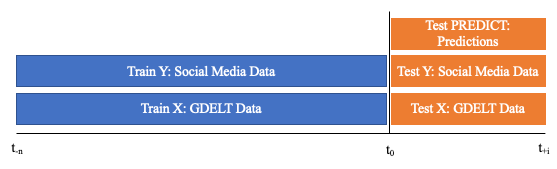
\includegraphics[width=\columnwidth]{PredictGraph.png}
\caption{Conceptual View of the Prediction Process} 
\label{PredictGraphFigure} 
\end{figure}

\par In the canonical case, %of what? "in the canonical case of prediction, predict using the following", maybe
 a prediction is made using the following: X-Train is compared to Y-Train to establish the relationship between them (e.g., a linear correlation). Then, X-Test is used to create a time series for the testing period; this is termed the Y-Predict. It is then possible to score the performance of the prediction by comparing Y-Predict with the Y-Test values, which contain the `correct' answer.

\par This can represent this as a function:

\begin{equation}
  Y_{predict} = f(Y_{Train},X_{Train},X_{Test})
\end{equation}

\par or

\begin{equation}
  y_{t0}, y_{t1}, y_{t2}, ... y_{ti} = f([y_{t-n}, ...y_{t-2}, y_{t-1}],[x_{t-n}, ...x_{t-2}, x_{t-1}],[x_{t0}, x_{t1}, x_{t2}, ... x_{ti}])
\end{equation}


\par While this is a canonical case, %of prediction?
 it is not the only case. For example, some predictions may need to be made without using X-Test. A true forecast into an unknown future, such as attempting to predict social media events days or weeks in advance, would be done without the values in X-Test, because the GDELT data in X-Test would also be unknown. In equation form:

\begin{equation}
  Y_{predict} = f(Y_{Train},X_{Train})
\end{equation}

\par Typically, the training period is longer than the prediction period. This is especially so in the second form, as predicting into the unknown without the X-Test values available is difficult.

\par The units for the time series values are usually `days', so that the series values are `events per day'. However, this can be changed and the series can be created for any unit of time (e.g., 4 hours). The limit is the resolution of the data. In GDELT, the event data are identified by the `day' field, which is a calendar date with no meaningful time stamp; however, the field \textit{dateadded} field can be used, and this has a 15-minute resolution. The dateadded field can also be more appropriate if what is being examined is the relationship between the dependent variable (e.g., social media data) and the appearance of an event in the news rather than the event itself---that is, when the event was being discussed in the news and not when the event actually happened.

\section{Prediction Methods}
\subsection{Raw}
\subsection{Base Values}
\section{Replay}
 A category of predictions known as \textbf{replay} has a simple idea: take values from the training period and repeat them in the testing period.
\par Variations on this theme are possible. For example, given the need to predict 8 days into the future, one could simply replay the 8 days immediately prior to $t_0$. Alternatively, one could align the days being replayed by day of the week, to catch weekly cycles of high and low activity.

\subsection{Linear Regression}
\subsubsection{Linear Regression Weighted}

\section{Long Short-Term Memory}


\section{Elastic Net}
\section{Gradient Boost}
\section{Lasso}
\section{Adding Prediction Methods}
\subsection{Java}

\par Creating new prediction methods in Java is straightforward: All prediction classes must implement 
\subsection{Python}




%!TEX root =  GDELT_GA_Search_UsersManual.tex

\chapter{Scoring Methods} \label{chap:ScoringMethods}

\section{Root Mean Square Error (RMSE)}
\section{Normalized Root Mean Square Error (NRMSE)}
\subsection{Mean}
\subsection{MinMax}
\subsection{Standard Deviation}
\section{Correlation (Positive Only)}
\section{Input Correlation}
\subsection{Trimmed}
\subsection{Positive Only}
\section{Adding Scoring Methods}
\subsection{Python}
\subsection{Java}


% %!TEX root =  GDELT_GA_Search_UsersManual.tex

\chapter{Preparing Input Data} \label{chap:PreparingInputData}
%Note sure about location: Blueberry graph needed. Cameo codes are 4-digit codes. The first two are root codes (1-20) and the second two are sub-divisions of root codes (i.e., subtype). Goldstein is the range of how 'nice' an event is based on the cameocode. Cameo code is represented on the x-axis and Goldstein is represented on the y-axis. Negative values (-) signify 'bad' and positive values signify 'good'. Re: "Spatial Tuning" (ch?) reconfigure Goldstein values and cameo codes because the numbers go from neutral to good and then bad.
\section{Input Data Overview}

The types of input data needed are:
\begin{itemize}
\item GDELT data 
\begin{itemize}\item Events Table \item Mentions Table\end{itemize}
\item Time series data for comparisons
\item Any other parameter configurations (TBD!)
\end{itemize}

\par These will have a preferred file location ('data' directory in the GDELT\_GA\_Search project), although users can probably override this.

\section{GDELT Data}
Description
\subsection{Events Table}
\par \textbf{GlobalEventId} is the link between this table and the Mentions Table (see \hyperlink{section.4.2}{Mentions Table} section). \\GDELT can infer multiple events from a single real-world event, so a single event in the real-world can show as multiple lines in this table. For example, if Norway and Namibia had a simple bilateral meeting (Norway$\leftrightarrow$Namibia), there could be two entries for the same event: one entry for Norway$\rightarrow$Namibia and another for Namibia$\rightarrow$Norway. Similarly, if Norway, the Netherlands, and Namibia had a conference, there could be multiple entries for Norway$\rightarrow$Netherlands, Netherlands$\rightarrow$Namibia, and Norway$\rightarrow$Namibia. \emph{Having multiple entries skews event counts}, but it can also be useful.

\par \textbf{FileName} is not relevant (FOR WHAT?). It only relates to how data are distributed %(DISTRIBUTED WHAT/WHERE? "relates to data distribution" HIDES MISSING INFORMATION BETTER).

\par \textbf{DateAdded} is when GDELT found the record %(WHAT RECORD? THE MEDIA COVERAGE?). DateAdded may("is"? WHY WOULD IT NOT BE?) be the best indication of when media about an event is released.

\par \textbf{FractionDate} is a representation of the \emph{date} as a fraction of the year. It does \emph{not} state the time. It can be used for sorts %(PREFERRED JARGON TO 'SORTING'?). 
\\It is easier to parse DateAdded than FractionDate, so using a ‘Date’ object is better. %(FROM DateAdded or below? BETTER HOW—FOR SORTS?). 

\textbf{Day}, \textbf{MonthYear}, and \textbf{Year} are similar. %(IN WHAT WAYS? WHY DOES THIS MATTER? ARE THESE DATE OBJECTS?)


\subsubsection{CAMEO Codes}
There are four \emph{Conflict and Mediation Event Observations Event and Actor Codes}, or CAMEO Codes, in GDELT:
\begin{itemize} \item QuadClass \item EventRootCode \item EventBaseCode \item EventCode \end{itemize}

\par  For information outside of the scope of this introduction, visit the CAMEO dictionary, \href{http://data.gdeltproject.org/documentation/CAMEO.Manual.1.1b3.pdf}{CAMEO Conflict and Mediation Event Observations Event and Actor Codebook}.

\par \textbf{QuadClass} is the broadest %(IN TERMS OF RESOLUTION?) 
and has four values: 1=Verbal Cooperation, 2=Material Cooperation, 3=Verbal Conflict, 4=Material Conflict.

\par \textbf{EventRootCode} is a 1- or 2- digit marker ranging from 1 to 20. (These are explained below.)

\par \textbf{EventBaseCodes} are finer resolution. %(WHAT DOES RESOLUTION REFER TO?)

\par \textbf{EventCodes} are the finest resolution.

\subsubsection{EventRootCode}
There are twenty \textit{root code} markers and their categories: 
\begin{enumerate} \item MAKE PUBLIC STATEMENT \item APPEAL \item EXPRESS INTENT TO COOPERATE \item CONSULT  \item ENGAGE IN DIPLOMATIC COOPERATION \item ENGAGE IN MATERIAL COOPERATION \item  PROVIDE AID \item  YIELD \item  INVESTIGATE \item DEMAND \item DISAPPROVE \item REJECT \item THREATEN \item PROTEST \item EXHIBIT MILITARY POSTURE \item REDUCE RELATIONS  \item COERCE \item ASSAULT \item FIGHT \item ENGAGE IN UNCONVENTIONAL MASS VIOLENCE \end{enumerate} 

\par Root codes are a total of four digits. %I don't understand the difference between CAMEO codes and root codes, although I recognize that the clip from the GDELT codebook at the top of page 3 here: https://docs.google.com/document/d/1nPShaMtQuO797W3OXe03_icMVnR_wfZlJ4ILYlpa65I/edit

The first two digits are the event root codes which mark the broader category and the second two digits mark the subcategory. 
For example, code “1424” is “Conduct hunger strike for change in institutions, regime”—a subtype of ‘Protest’. Similarly, code 0251 is "Appeal for easing administrative sanction," which is a subtype of 'Apeal'. %but also something about three digit codes?

\par \href{https://docs.google.com/spreadsheets/d/1z2bK0SD826bL5eq-5ZhLCF3rnJoVnW_fJS1wBEAx03Y/edit?usp=sharing}{An account of the codes and the number of events in each code can be found here.}

\par For example, Base Code ‘20’ has only a total of 141 events out of the ~600K in the data set.

The implication of this is that some changes to queries are different from others. For instance, if the query allows “018”, there are only ~500 events.
If it expands to include ‘019’, this will only add 31 new events.
If it expands to include ‘017’, this will add ~1600 events, causing the number of events to quadruple. 
Search cost is high, and exploring whether there is a change when 31 events are added to a search is unlikely to yield anything interesting, so the priority should be on the highest event counts. %what are these three digit codes exactly? Event Base Codes?

\subsubsection{WhatToCallThisSection?} 
There are seven fields that refer to the original text article or articles from which the event was derived:
\begin{itemize} \item sourceurl \item sourceurl\_h \item AvgTone \item IsRootEvent \item NumArticles \item NumMentions \item NumSources \end{itemize}

\par The \textbf{sourceurl} and \textbf{sourceurl\_h} are both URLs.
The \_h version is the \emph{hashed} version that will match any reference in our larger tweet data set.
\\The article identified in the sourceurl field should be in the Mentions Table (see \hyperlink{section.4.2}{Mentions Table} section.)
This article is the first article in which an event was identified.
 
 \par \textbf{AvgTone} is the average \emph{tone} of articles, but all of these will (in theory) be in the \hyperlink{section.4.2}{Mentions Table}. %What exactly is tone here? Is tone about a text's attitude towards an event? Is it measured in relation to some stab at objective gravity/levity of an event?
 
 \par \textbf{IsRootEvent} is true if the event was detected in the first paragraph of the document in source\_url. (Not to be confused with ‘Root Code’.) It is not updated if other sources in the \hyperlink{section.4.2}{Mentions Table} refer to it in column 1. %What is meant by 'true'? Is IsRootEvent not true if other sources refer to it in column 1? 
 
\par \textbf{AvgTone}, \textbf{NumArticles}, \textbf{NumMentions}, and \textbf{NumSources} are all fields that need to be used with caution. 
 They only refer to articles captured “During the 15-minute Update” in which it was first seen. 
 This is not ‘Within 15 minutes of it being seen’; it is cut off strictly at 15-minute intervals. %what is 'it' exactly?
 For example, an event that first appears at 12:01 AM could be seen more times before 12:15, whereas one first seen at 12:14 would only have one minute to acquire more mentions. 
 This does not relate to the time that the article appears; it relates only to the time that GDELT found it.

\textbf{\textit{Basically, all of these fields are now better addressed by considering the \hyperlink{section.4.2}{Mentions Table} directly, with IsRootEvent being lost entirely.}} %does this mean they should be ignored? Have they been replaced? How can we warn our readers that the above list isn't as important as the following list?

\subsubsection{Actor Codes}%I'm guessing at the section name here
\begin{itemize} \item Actor1Code / Actor2Code
\item Actor1CountryCode / Actor2CountryCode
\item Actor1Geo\_ADM1Code / Actor2Geo\_ADM1Code
\item  Actor1Geo\_ADM2Code / Actor2Geo\_ADM2Code
\item Actor1Geo\_CountryCode / Actor2Geo\_CountryCode
\item Actor1Geo\_FeatureID / Actor2Geo\_FeatureID
\item Actor1Geo\_FullName / Actor2Geo\_FullName
\item Actor1Geo\_Lat / Actor2Geo\_Lat
\item Actor1Geo\_Long / Actor2Geo\_Long
\item Actor1Geo\_Type / Actor2Geo\_Type \end{itemize}
%explanations? actors are involved parties is an event? how is who is Actor1 and Actor2 decided? 

There is a unique code for each actor from the \href{http://data.gdeltproject.org/documentation/CAMEO.Manual.1.1b3.pdf}{CAMEO dictionary}.

Here is a breakdown of most common Actor1 Codes and the number of events:
%should we have a clear agent key or note the agents here?
\begin{enumerate}  
\item 132852	\quad VEN
\item 68825	\quad GOV
\item 47030	\quad null
\item 45833	\quad USA
\item 24318	\quad RUS
\item 23465	\quad VENGOV
\item 18520 	\quad COL
\item 17325	\quad MIL
\item 12800	\quad OPP
\item 10602	\quad LEG
\item 8748		\quad BRA
\item 7893		\quad CVL
\item 7764		\quad MED
\item 7366		\quad BUS
\item 7229		\quad USAGOV
\item 7150		\quad ESP
\item 6921		\quad PER
\item 6390		\quad CHN
\item 5986		\quad COP
\item 4852		\quad VENMIL
\item 4636		\quad CUB
\item 4536		\quad CAN
\item 4531		\quad MEX
\item 4299		\quad IGOUNO
\item 4242		\quad VENOPP 
\end{enumerate}

Here is a breakdown of the most common Actor2 Codes and the number of events in which they appear:

\begin{enumerate}
\item 142495	\quad VEN
\item 128720	\quad null
\item 56931	\quad GOV
\item 36518	\quad USA
\item 23306	\quad VENGOV
\item 17706	\quad MIL
\item 17634	\quad COL
\item 13768	\quad RUS
\item 12428	\quad OPP
\item 8370		\quad LEG
\item 7896		\quad BRA
\item 7321		\quad CVL
\item 6264		\quad BUS
\item 6161		\quad MED
\item 5181		\quad PER
\item 5085		\quad USAGOV
\item 5067		\quad ESP
\item 4587		\quad COP
\item 4292		\quad VENMIL
\item 4093		\quad CHN
\item 4082		\quad VENOPP
\item 3723		\quad IGOUNO
\item 3519		\quad CUB
\item 3470		\quad EUR
\item 3460		\quad URY
\item 2900		\quad MEX
\item 2757		\quad CAN
\item 2642		\quad VENCVL
\item 2354		\quad TUR
\item 2316		\quad JUD
\item 2054		\quad VENLEG
\item 1978		\quad USAMED
\item 1967		\quad COLGOV
\end{enumerate}

\subsubsection{Mutation} %guessing at the section name
In thinking about how use actors in a \textbf{mutation}, %defined how?
 imagine that a query includes a set of these already:

\textbf{Actor 1 {\scriptsize E} {\large \{ VEN, GOV, USA, VENGOV \}}}  

To \emph{mutate} this, it is possible to:
\begin{itemize}
\item Remove one of the actor codes
\item Add another actor code
\item Replace an actor code by removing one and adding another 
\end{itemize}

\par Use the counts of events in the overall data set to guide which actor codes would be removed or added. 
\\ In order to do this, keep data for the weighted selection. %"to do this" meaning "mutation" or something else?
\par Note that adding more actor codes should be less likely as the set gets large.
Consider whether the set is a set of records should be included or excluded. %What determines the decision? i.e. what goals?
Also consider using the other codes %Like what? The sourceurl, AvgTone, IsRootEvent, etc. from the above section?
 because they can capture the same information but more broadly and sometimes more reliably.
 
 \subsubsection{CrypticCodes}%change section title
 Other codes are more cryptic. Here is \textbf{Actor1Geo\_FeatureID} with counts of occurrences:
\begin{enumerate}
\item 157753 \quad VE
\item 113901 \quad -938457
\item  47292 \quad null
\item  32221 \quad 531871
\item  22163 \quad US
\item  15568 \quad -2960561
\item  15447 \quad CO
\item  11759 \quad RS
\item  9555 \quad BR
\item  9334 \quad -960192 \end{enumerate}
%Should we say to ignore geo location? refer to p.8, GDELT manual part  "Actor1Geo_FeatureID" to try to make sense of this: https://docs.google.com/document/d/1nPShaMtQuO797W3OXe03_icMVnR_wfZlJ4ILYlpa65I/edit

A few entries do have some of the other data described in the GDELT book.%this? http://data.gdeltproject.org/documentation/CAMEO.Manual.1.1b3.pdf

For example, a few thousand have \textbf{Known Group ID}:

 \begin{enumerate} 
 \item 629981\quad null
\item   5364 \quad UNO
\item   2234 \quad EEC
\item    691 \quad IRC
\item    508 \quad OPC
\item    265 \quad NAT
\item    142 \quad ICC
\item    116 \quad HRW
\item    112 \quad OAS
\item     93 \quad WEF
\item     88 \quad IMF
\item     76 \quad TAL
\item     70 \quad AMN
\item     53 \quad ICG
\item     27 \quad IOM
\item     20 \quad SAD
\item     13 \quad ITP
\item     10 \quad ALQ
\item       8 \quad SCE
\item      8 \quad ARL
\item      7 \quad ASN
\item      6 \quad IPU
\item      5 \quad XFM
\item      5 \quad MSF
\item      4 \quad WTO
\item      3 \quad WAS
\item      2 \quad GOS
\item      2 \quad GOE
\item      2 \quad COE \end{enumerate}

A few even have \textbf{Religion1Code}. %meaning what?
However, it’s a bit unclear if this adds more information above the actor codes (so, the same actor should always have the same code).








\subsection{Mentions Table}
Using the Mentions Table %explain
\par The mentions table has the following fields:
\begin{itemize} \item \textbf{GlobalEventId} - Key that links this to the events table
\item \textbf{EventTimeDate} - Date/Time of the original event
\item \textbf{MentionIdentifier} - URL
\item \textbf{MentionSourceName} - Domain
\item \textbf{MentionTimeDate}  
\item \textbf{MentionDocTranslationInfo} - Which articles were translated from Spanish %other langs too?
\item \textbf{MentionDocLen}
\item \textbf{MentionDocTone}
\item \textbf{Extras}
\item \textbf{MentionType}: Always ‘1’ in the data set
\item \textbf{SentenceId}
\item \textbf{Actor1CharOffset}
\item \textbf{Actor2CharOffset}
\item \textbf{ActionCharOffset}
\item \textbf{Confidence}
\item \textbf{InRawText} \end{itemize}

\textbf{Extras} is always null. \textbf{Translation information} is only present for articles that were translated.
\par A generalized structure is needed for a field in queries. This is what is currently used:
%insert picture from Doc p.10 or figure out font formatting
\par While this works, it requires hard-coding every element and does not allow for explorations.
\par Take these two as examples. %these two what? are they in the picture?
They are different in a couple of important ways: 
\begin{enumerate} 
\item One is a continuous value (here a double), and the other is an integer.
\item One ranges from -10.0 to +10.0; the other can be zero or above, without any limit \footnote{There is no limit in theory, but in practice there will be an unknown maximum value in the data set.}.
\end{enumerate}
\par Think of these as domains to explore. Next, think about how to explore them. Here are some beginning operations to consider:
\begin{enumerate} \item \textbf{Initialize} the field in an intelligent way. This can be done by including all elements (e.g., starting with -10.0 $\leftarrow$ x $\leftarrow$ 10.0 for Goldstein, which will include all entries).
\item \textbf{Reduce} the scope of the field. Here is how this is done:
\begin{enumerate}\item Raising the minimum value (e.g., -7.0 $\Leftarrow$ x $\Leftarrow$ 10.0)
\item Reducing the maximum value (e.g. -10.0 $\Leftarrow$ x $\Leftarrow$ 7.0)
\item Both \end{enumerate}\end{enumerate}

It is also possible to split the range so that there are two: %two what?
(-10.0 $\Leftarrow$ x < -7.0 \& -7.0 $\Leftarrow$ x $\Leftarrow$ 10.0)

Notice that there is an issue with inclusive/exclusive ranges. In the first, the -7.0 is exclusive, but in the second the -10.0 is inclusive. In general, use the lower bound as inclusive but the upper bound as exclusive. Note that this means that if x < 10.0 is used, all values of 10.0 exactly are omitted.


All of these can be thought of as operations:

\begin{enumerate} \item \textbf{InitFullRange} - Initialize but include all records
\item \textbf{InitRandomRange} - Initialize but include a random range
\item \textbf{Reduce} - Reduce the range
\item \textbf{Expand} - Expand the range
\item \textbf{Split} - Cut into two distinct pieces that together capture all of the original domain
\item \textbf{Invert} - Make so that all excluded become included \end{enumerate}

This is a good set to start with. One of the advantages is that it can be used with either numerical or unordered sets.



\section{Time Series Data for Comparisons}\label{TimeSeriesDataStructure}
The data required for time series comparisons have a simple structure:

\begin{lstlisting}
platform,frame,ConvertedDate,counts
twitter,capitol,2020-10-01,1034
twitter,capitol,2020-10-02,1081
twitter,capitol,2020-10-03,1096
twitter,capitol,2020-10-04,1116
twitter,capitol,2020-10-05,1198
twitter,capitol,2020-10-06,1234
twitter,capitol,2020-10-07,1271
twitter,capitol,2020-10-08,1368
etc.
\end{lstlisting}

The first column is the source of the data (typically called the `platform'); the second is a topic (commonly called the `frame'). The third is a date in the format shown, and the fourth is the value associated with that date.

Generally this file will cycle through multiple frames and then multiple platforms, if any, repeating the same dates.


% %!TEX root =  GDELT_GA_Search_UsersManual.tex

\chapter{Spatial Tuning}
\label{chapter:SpatialTuning}

\textbf{Spatial Tuning} means customizing the way the search algorithm explores a particular dimension.
For example, two fields that are present in the GDELT event data are \textit{latitude} and \textit{longitude}.
When parsing the GDELT data, the gdelt\_ga\_search algorithm separates events by geographic location.
This is done with a simple mathematical approach: latitude and longitude are used to form a `box' on the 
Earth's surface. 
Events are categorized as either \textit{inside} or \textit{outside} that box. 
It is possible to expand and shrink the box for the purpose of growing or shrinking the number of events found \textit{inside} the search region.

\par Events in a data set are not evenly distributed on the Earth's surface. 
Of areas that have events, some contain a large or small number of events.
Small areas with many events are \textit{high-density} areas, while areas with few events are \textit{low-density areas.}
Of course, there are places without events. 
For example, there are virtually no events that occur in the middle of the Pacific Ocean. 
Many other areas do not have events, which can be seen in data sets for specific geographic regions. 

\par Exploring areas that are not represented in the data set can waste time. If there are no events in a region, the region can be disregarded.

\par If events are low-density in some areas and high-density in other areas, use a more nuanced strategy. 
For a box with mostly low-density areas, use large increases (i.e, expand the box by hundreds of miles) to include a few more events by expanding the size of the search box.
For a box with mostly high-density areas, use small increases (i.e., expand the box by a few miles). Small increases may need to be done multiple times. 
If moving the boundaries even a few miles means including or excluding thousands of events, then a better strategy is to use small icreases.

\par The above logic applies to other fields in the GDELT data. One of the other GDELT fields is /textit{Root Code}, which has values from 1 to 20. 
Just as events are subsetted by latitude/longitude, codes can also be used to subset the data set.
For an example with only one dimension (so instead of a 2-D box there is only a range), consider a search range with event codes 7 through 11.

\par To expand the search for more event types, the code range could be expanded by moving one of the boundaries. For example, the range could expand to 6-11 or  to 7-12, or by moving both of the boundaries, to 6-12.

\par The search can also be made smaller by restricting the code range. 
Using the above example, to search for fewer event types, the range could be decreased to 8-11, 7-10, 3-8, etc.

\par However, if it is known that there are no events labeled by a specific code, then that code should be skipped. 
Using the above example of the range 7-11, if there are no code `6' events, then there is no reason to search for '6'. Instead, it is better skip 6 and use 5-11 instead of 7-11.

\par Spatial tuning refers to the collection of strategies to optimize the way that the gdelt\_ga\_search algorithm expands and restricts its search ranges on specific domains, given what is known \textit{a priori} about the distribution of events on those domains in a data set.


% %!TEX root =  GDELT_GA_Search_UsersManual.tex

\chapter{Designing Tests} \label{chap:DesigningTests}

\section{Number of Generations}
\section{Population Size}
\section{Stop Conditions}
\section{Preparing Initial Queries}

%!TEX root =  GDELT_GA_Search_UsersManual.tex

\chapter{Downloading GDELT Data} \label{chap:DownloadingGDELTData}

\section{Using the Events and Mentions Scrapers}

\gdgas includes a pair of tools to allow you to acquire GDELT data. The \textit{GDELT\_Events\_Scraper} tool downloads GDELT Event data; the \textit{GDELT\_Mentions\_Scraper} downloads GDELT Mention data. Downloading Mention data is a second step that relies on an existing corpus of event data; when downloading mentions, only mentions associated with events in the events corpus are stored.

Running these tools is best done in an IDE; they are not currently configurable from the command line, and the code must be changed to download specific subsets of data. The result of these tools is a file (user-specifiable, but customarily either GDELT\_Events\_Data.csv or GDELT\_Mentions\_Data.csv) that contains the GDELT data. The data are in the standard GDELT format; they are not transformed. For historical reasons, the Mentions file has a header line, while the Events file does not.

GDELT data is stored online in a repository of ZIP files that are identified by a time stamp code. The tools here are given a start and end time range and move from beginning to end, downloading the files, unzipping them, and assembling the results into a file that can be used as \gdgas input. The ZIP files can optionally be retained or deleted; retaining them allows the routine to be run again without hitting GDELT's servers, but the files are quite large to store.

\section{Setting download parameters}
Each of the tools allows you to specify the date/time range of files to be downloaded, and a few other options. In total the options are:

\begin{itemize}
\item startTime The earliest file to download (inclusive)
\item endTime The latest time to download (not inclusive; the routine stops before downloading this file.)
\item dataPath A path to directory in which the data output will be stored.
\item ZIP\_PATH\_ROOT the path to the directory in which the ZIP files will be stored when downloaded (and optionally retained)
\item LoopLimit A debug fail-safe to stop from downloading too many files; this is in place because the files are very large and you may want to stop downloading at some specific point (but this could also be limited by the time ranges)
\item keepZip True if the ZIP files should be kept; false if they should be automatically deleted once expanded
\item fileName The name of the file that will be created
\item appendToFile True if the output file should be appended to; false if it should be deleted before writing begins.
\item sleepInterval An interval in milliseconds that the routine should wait between downloading files. This is to ensure that the server does not believe it is being attacked. The default is 500. Reducing it can lower the total time the routine needs, but the response of GDELT's servers to faster downloads is not known.
\end{itemize}

Additionally, the Events scraper has  parameter (`PROB') that can be set to a number lower than one; this will probabilistically exclude lines from the original files. This is a crude form of random sampling. If set to zero and the keepZip parameter is set to true, the routine effectively downloads GDELT ZIP files and does no other action.

The Mentions scraper has an additional required parameter that gives the path and name of the Events table to used to create the GDELT corpus; only mentions related to events in the corpus are loaded.

\section{Filtering Events}
The code can be modified to download only include specific events. Line 114 in the Events scraper includes an example. Filtering would have to be done in a customized way and is not covered in detail here.

\bibliographystyle{plain-annote}
\bibliography{mybibliography}


\end{document}
\end

